\NeedsTeXFormat{LaTeX2e}
%\PassOptionsToClass{handout}{beamer}
\documentclass{beamer}
\usepackage{beamerPack}
\usepackage[boxed,ruled,vlined]{algorithm2e}
\usepackage{setspace}
\usepackage[05]{../lecture}
\def\x{\hspace{4.1ex}}    %BETWEEN TWO 1-DIGIT NUMBERS
\def\y{\hspace{3.4ex}}  %BETWEEN 1 AND 2 DIGIT NUMBERS
\def\z{\hspace{2.7ex}}    %BETWEEN TWO 2-DIGIT NUMBERS
\subtitle{動的計画法}
\begin{document}

\begin{frame}[fragile]{}
\titlepage
\end{frame}

\begin{frame}[fragile]{素朴なアルゴリズムと巧妙なアルゴリズムの違い}{}
\begin{itemize}%\itemsep8pt
\item 時間計算量を減らす:無駄を省く
\item 空間計算量を減らす:無駄を省く
\end{itemize}

\vfill
空間計算量を減らす例は前回出てきたpartition。元々は一つの配列から二つの配列に要素をコピー(移動)させるアルゴリズムだったが、効率を追求した結果、あのようなプログラム定義になった。
\end{frame}

\begin{frame}[fragile]{素数の計算}{}
この話は相似問題に等価なものが含まれるので削除する話なので、今回の最後か次回がふさわしい。
\end{frame}

\section{for programmers}		%%%%%%%%
\subsection{}

\begin{frame}[fragile]{数学的解析の力}{}

\[
Fib(n) = \frac{1}{\sqrt{5}}
\left\{
\left(\frac{1 + \sqrt{5}}{2}\right)^n
-
\left(\frac{1 - \sqrt{5}}{2}\right)^n
\right\}
\]

\end{frame}

\begin{frame}[fragile]{ふかしぎおねえさん}{}
a
\end{frame}

\section{dynamic programming}		%%%%%%%%
\subsection{}

\begin{frame}[fragile]{動的計画法}{}
\begin{block}{動的計画法(dynamic programming)}
\begin{itemize}%\itemsep8pt
\item 再帰的に分割された部分問題の(最適)解から元問題の(最適)解を構成
\item 部分問題の重複性の利用
\end{itemize}
\end{block}

\footnotetext{線形計画法は不等式に関する問題}
\end{frame}

\section{algorithm design}		%%%%%%%%
\subsection{}


\begin{frame}[fragile]{重複を避ける}{フィボナッチ数}
\begin{codeof}{language=Rust}{}
fn fib(n: usize) -> usize {
    let mut memo = [0; 10000];
    fn f(n: usize) -> usize {
        if n < 2 { return 1; }
        if memo[n] != 0 { return memo[n]; }
        let result = f(n - 2) + f(n - 1);
        memo[n] = result;
        result
    }
    f(n)
}
\end{codeof}
f(n-1)の計算がf(n-2)の計算を含んでいる$\to$重複問題の出現。

\end{frame}

\begin{frame}[fragile]{空間計算量を下げる}{フィボナッチ数}
\begin{codeof}{language=Rust}{方向の逆転}
fn fib(n: usize) -> usize {
    fn f(k: usize, memo1: usize, memo2: usize) -> usize{
        if n == k { return memo1 + memo2; } 
        f(k + 1, memo2 + memo1, memo1);
    }
    if n <= 2 { 1 } else { f(3, 1, 1) }
}
\end{codeof}

\begin{codeof}{language=Rust}{どうしても再帰がわからない人向け(実行時間は変わらない)}
fn fib(n: usize) -> usize {
    if n <= 2 { return 1; }
    let (mut memo2, mut memo1) = (0, 0);
    for k in 2..n {
        (memo1, memo2) = (memo2 + memo1, memo1);
    }
    memo1 + memo1
}
\end{codeof}
\end{frame}

\begin{frame}[fragile]{素数判定}{}
\[
\forall k \in [2, n-1] : n \% k \ne 0.
\]

\begin{codeof}{language=Rust}{$O(N)$}
fn is_prime(n: usize) -> bool {
    for i in 2..n-1 {
        if n % i == 0 { return false; } 
    }
    true
}
\end{codeof}
高速化
\begin{enumerate}%\itemsep8pt
\item 偶数は調べない
\item 素数しか調べない(そのためにはn以下の全ての素数をまず調べないといけないのだが)
\end{enumerate}
\end{frame}

\begin{frame}[fragile]{素数判定:重複を省く}{}
\[
\forall k \in [2, n-1] : n \% k \ne 0.
\]

\begin{itemize}%\itemsep8pt
\item 6000が2で割れた。3000でも割れる。
\item Xがkで割れた。$\to$ X/kでも割れる。
\item Xがkで割れなかった。$\to$ X/kでも割れない?
\item Xがkで割れるなら$\to$ X/kでも割れなければならない。
\end{itemize}

\[
\forall k \in [2, \lceil\sqrt{n}\rceil] : n \% k \ne 0.
\]

\[
O(n) \to O(\sqrt{n})
\]
\end{frame}

\begin{frame}[fragile]{問題の再帰構造の次元を落とす(線形化)}{}
どんな例を用意していたのか思い出せない。
\end{frame}

\begin{frame}[fragile]{動的計画法}{}
ここでこの術語を出すのがいいかどうか。
\end{frame}

\begin{frame}[fragile]{メモ化}{
%\href{https://ja.wikipedia.org/wiki/%E3%83%A1%E3%83%A2%E5%8C%96}%
%{\beamergotobutton{wikipedia}}
}

X型の引数からY型の計算結果を求める関数に対してXからYへのメモを作ることで時間計算量を減らす
\begin{codeof}{language=Rust}{メモ化の一般形}
fn foo (問題指定) -> 解の型 {
  static memo: Hash<問題指定の型, 解の型>;
  // メモの確認
  if memo[問題指定]が有効な値を持つ {
    return memo[問題指定];
  }

   本来の計算:問題指定から解を求める

  // メモする
  memo[問題指定] = 解;
  return 解;
}
\end{codeof}

\footnotetext[1]{定型化されているので言語によってはこのコードを自動生成する}
\end{frame}

\begin{frame}[fragile]{fibに対するメモ化の例}{
%\href{https://ja.wikipedia.org/wiki/%E3%83%A1%E3%83%A2%E5%8C%96}{\beamergotobutton{repl it}}
}
\begin{codeof}{language=Rust}{fib (memo.rs)}
pub fn fib(n: usize) -> usize {
    if let Ok(hash) = MEMO.read() {
        if let Some(r) = hash.get(&n) {
            return *r;
        }
    }
    let n_1 = if n <= 2 { 1 } else { fib(n - 1) };
    let n_2 = if n <= 2 { 0 } else { fib(n - 2) };
    let result = n_1 + n_2;
    if let Ok(mut hash) = MEMO.write() {
        hash.insert(n, result);
    }
    result
}
\end{codeof}

\begin{spacing}{0.7}\fontsize{6}{6}\selectfont
メモは毎回初期化されないようグローバル(static)変数にしたい。
Rustではグローバル変数への操作は同期操作を使ったスレッド安全なものしか受け付けないので、
ライブラリのインポートや変数定義(ここでは省略)、アクセス(L.2--6, L.10-12)が面倒になっている。
\end{spacing}
\end{frame}

\begin{frame}[fragile]{効果の確認}{}

\begin{codeof}{language=Rust}{}
fn main() {
    let n = 46;
    // mainから1回しか呼ばなくても再帰しているのでメモ化は有効
    println!("fib({:>2}) = {:>11}", n, fib(n));
    println!("fib({:>2}) = {:>11}", n, slow_fib(n));
    // メモに残っているので同じ計算では2回目以降はO(1)
    for i in 30..=48 {
        println!("fib({:>2}) = {:>11}", n, fib(n));
        println!("slw({:>2}) = {:>11}", n, slow_fib(n));
    }
    // 引数が違ってもメモに残っているので新規分だけ計算
    for i in 30..=48 {
        println!("fib({:>2}) = {:>11}", i, fib(i));
        println!("slw({:>2}) = {:>11}", i, slow_fib(i));
    }
}
\end{codeof}
\end{frame}

\begin{frame}[fragile]{最短経路}{}

経路数ではなく最短経路を求めよ。ただし。
\end{frame}

\begin{frame}[fragile]{最短経路2}{}
経路数ではなく最短経路を求めよ。
\end{frame}

\begin{frame}[fragile]{ダイクストラ法}{
%\href{https://ja.wikipedia.org/wiki/ダイクストラ法}{\beamergotobutton{wikipedia}}
}
\begin{quotation}
\fontsize{9}{12}\selectfont
最短経路問題は、ビー玉と紐を用いて解くことができる。
まずビー玉を頂点、紐を辺にするグラフを工作する。
グラフを板の上に置き、スタートの頂点にあたるビー玉だけをつまむ。
グラフが置かれている板を取り除くと、グラフは自由落下を始めるが、スタートにあたるビー玉を持っているので、スタート地点から近いビー玉から順に落下が止まる。
ゴールにあたるビー玉が止まったとき、ゴールにあたるビー玉はスタートにあたるビー玉まで紐で一直線で結ばれている。
この直線が最短経路である。

ダイクストラのアルゴリズムは、上述の解法をコンピュータ上でシミュレートしたものである。
\end{quotation}
\end{frame}

\begin{frame}[fragile]{ダイクストラ法の根幹:相似問題の考え方による説明}{中間目標を設定し相似問題に帰着させたい}
中間目標の選択:どの頂点が確定できるか
\begin{itemize}\itemsep8pt
\item 距離確定頂点から最も「近い」未確定頂点とする
\begin{itemize}%\itemsep8pt
\item なぜならこの頂点に限り三角不等式が成立するから

\begin{center}
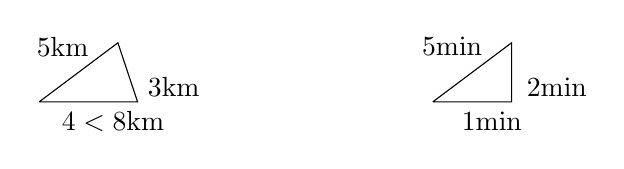
\begin{tikzpicture}[scale=0.25]
\draw (0, 0)
    -- (4, 3) node[near end, above=4pt, anchor=east] {$5$km}
    -- (5, 0) node[near end, right=2pt] {$3$km}
    -- (0, 0) node[near start,below] {$4<8$km};
\draw (20, 0)
    -- (24, 3) node[near end, above=4pt, anchor=east] {$5$min}
    -- (24, 0) node[near end, right=2pt] {$2$min}
    -- (20, 0) node[near start, below] {$1$min};
\end{tikzpicture}
\end{center}

\end{itemize}
\item この選択の余地の少なさが中間目標の変更を要請する
\begin{itemize}%\itemsep8pt
\item これまでの中間目標は終点から;今回は始点から
\end{itemize}
\end{itemize}

\vfill
相似問題:
\begin{itemize}\itemsep8pt
\item 頂点数が1減ったもの
\end{itemize}

\end{frame}

\begin{frame}[fragile]{時間が余るなら}{}
\begin{itemize}\itemsep8pt
\item 昇圧鎖 (Advent of Code year 2020 day 10)
\item 変態電卓 (Advent of Code year 2020 day 18)
\end{itemize}
\end{frame}


\section{Extra puzzles}		%%%%%%%%
\subsection{}

\begin{frame}[fragile]{問題3}{Advent of Code: year 2020, day 10}
\begin{enumerate}\itemsep8pt
\item 与えられた数列は以下の条件を満たす数列に変換できるか
\begin{itemize}%\itemsep8pt
\item 全ての項は、直前の項より1、2、または3大きい
\end{itemize}
\begin{enumerate}%\itemsep8pt
\item 数列1:\{ 16, 10, 15, 5, 1, 11, 7, 19, 6, 12, 4 \}
\item 数列2:もっと長い(91項)ので次ページに掲載
\end{enumerate}
\item 所与の数列に対し以下の条件を満たす数列の個数を求めよ
\begin{itemize}%\itemsep8pt
\item その列中の全ての項は、直前の項より1、2、または3大きい
\item 与えられた全ての項を使わなくてよい
\item ただし、所与の数列の最小項は必ず使うこと
\item ただし、所与の数列の最大項は必ず使うこと
\end{itemize}
\begin{enumerate}%\itemsep8pt
\item 先の数列1
\begin{enumerate}%\itemsep8pt
\item 求める数列は1で始まらなければならない
\item 求める数列は19で終わらなければならない
\item 例えば\{ 1, 4, 5, 7, 10, 12, 15, 16, 19 \}は条件を満たす
\item 網羅すると8通りあることがわかるので答えは8
\end{enumerate}
\item (64bit CPU所有者のみ)次ページの数列2
\end{enumerate}
\end{enumerate}
\end{frame}

\begin{frame}[fragile]{数列2}{toa04-p3-seq2.txt}
95
43
114
118
2
124
120
127
140
21
66
103
102
132
136
93
59
131
32
9
20
141
94
109
143
142
65
73
27
83
133
104
60
110
89
29
78
49
76
16
34
17
105
98
15
106
4
57
1
67
71
14
92
39
68
125
113
115
26
33
61
45
46
11
99
7
25
130
42
3
10
54
44
139
50
8
58
86
64
77
35
79
72
36
80
126
28
123
119
51
22
\end{frame}
\end{document}

